\begin{frame}{Đường ống dữ liệu}

\begin{figure}[H]
\centering
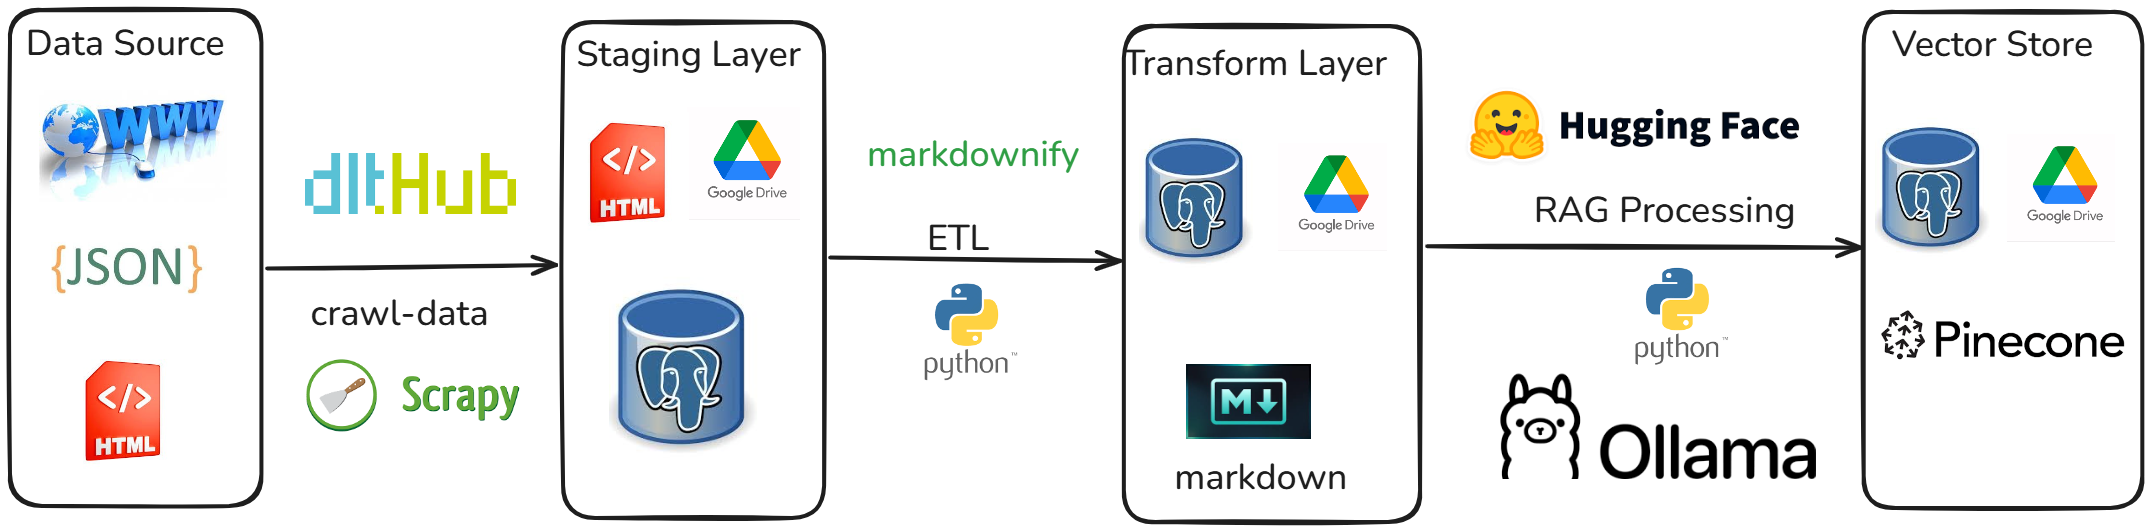
\includegraphics[width=\linewidth,height=0.275\textheight,keepaspectratio]{pictures/Data-Pipeline-VBPL.excalidraw.png}
\caption{Sơ đồ tổng quan đường ống dữ liệu VBPL (\footnotemark)}
\end{figure}

\begin{figure}[H]
\centering
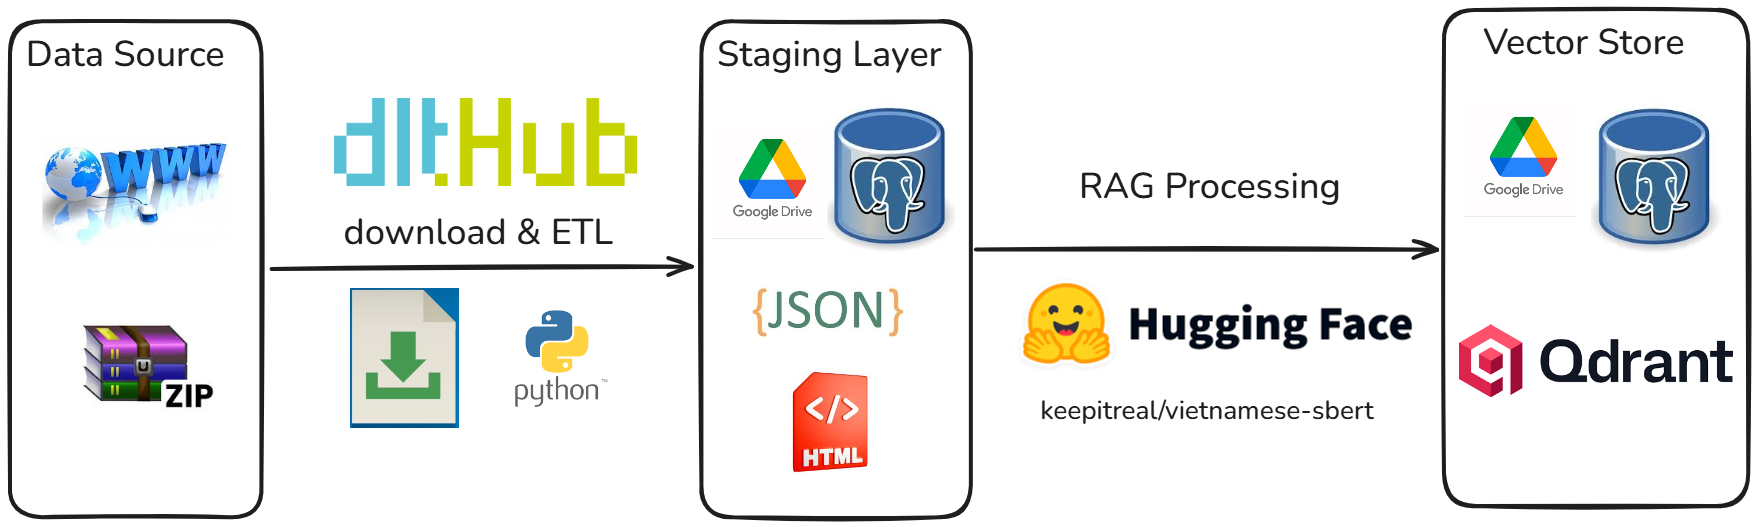
\includegraphics[width=\linewidth,height=0.275\textheight,keepaspectratio]{pictures/Data-Pipeline-PhapDien.excalidraw.png}
\caption{Sơ đồ tổng quan đường ống dữ liệu Pháp Điển (\footnotemark)}
\end{figure}

\footnotetext{\url{https://huggingface.co/keepitreal/vietnamese-sbert}}

\note{

đường ống dữ liệu văn bản pháp luật và pháp điển

quá trình tổng quan chung

đều dùng thư viện python để:

thu thập + xử lý + vector hóa dữ liệu
\hrule

từ nguồn dữ liệu ban đầu

cả 2 luồng dữ liệu đều sử dụng mô hình

nhúng embeddings trên huggingface là

% keepitreal
vietnamese-sbert có 768 chiều

cập nhật csdl tri thức của hệ thống
\hrule

đều có so sánh mã băm giúp tiết kiệm tài nguyên

}
\end{frame}
